\documentclass{sigchi}

\pagenumbering{arabic}

\usepackage{balance}  % to better equalize the last page

\usepackage{hyperref}
\usepackage[usenames,dvipsnames]{xcolor}
\usepackage[colorinlistoftodos]{todonotes}
\usepackage{soul}
\usepackage{amsmath}
\usepackage{xspace}

\setlength{\paperheight}{11in}

% %Needed to compile titlesec because IEEEtran does not define it
% \newcommand{\subparagraph}{} 
% \usepackage{titlesec}

% %Shrink the spacing after section headings a bit
% \titlespacing\section{0pt}{1.5ex plus 1ex minus 0.5ex}%
% {0.7ex plus 1ex minus 0ex}
% \titlespacing\subsection{0pt}{1.5ex plus 1ex minus 0.5ex}%
% {0.7ex plus .5ex minus 0ex}

\title{Will they synchronize? \\ The impact of background tempo on repetitive tasks\vspace{1.5ex}}

\numberofauthors{2}
\additionalauthors2
\author{
  \alignauthor Daniele Gallingani\\
    \affaddr{University of Illinois at Chicago}\\
    \email{dgalli3@uic.edu}\\
  \alignauthor Mingwei Li\\
    \affaddr{University of Illinois at Chicago}\\
    \email{mli53@uic.edu}\\
  \alignauthor Alessandro Panebianco\\
    \affaddr{University of Illinois at Chicago}\\
    \email{apaneb2@uic.edu}\\
  \alignauthor Gabriele Petronella\\
    \affaddr{University of Illinois at Chicago}\\
    \email{gpetro3@uic.edu}\\
  \vspace{2.0ex}
}

\newcommand{\testfirst}{Balloon Tapper\xspace}
\newcommand{\testsecond}{Balloon Inflater\xspace}

\begin{document}

\maketitle
% \listoftodos

\keywords{
	synchronization, music, tempo, activities, tablet interaction
}

\category{H.5.m.}{Information Interfaces and Presentation (e.g. HCI)}{Miscellaneous}

\terms{
    Synchronization; Measurement; Music
}

% !TEX root = main.tex
\section*{Abstract}

Music has  always represented an important factor in human lives. As the famous philosopher Friedrich Nietzsche said, "Without music life would be a mistake". Our body often seems to confirm this theory. In fact, during a normal daily routine we sometimes have to execute tasks while we are forced to listen to music coming from radios, computers, smartphones, etc. What we notice in these particular situations is that most of the times, in several activities, our body gestures end up trying to synchronize with the background music. With this paper we present data from an experimental study on synchronization to music. The study is based on an application for tablet devices that we have implemented. It is divided in two trivial activities: the first one, \textit{Balloon Tapper}, where the user has to tap a balloon that changes position in the screen every time is hit; the second one, \textit{Balloon Inflater}, where the user has to constantly tap a balloon in order to inflate it until, at some point, it explodes. Both of the tasks have to be performed  with and without music. Our main goal is to understand whether or not the user turns out to synchronize the performance of the two simple tasks with the offered music. Moreover, we want to analyze if the user is not only synchronizing with the music but even forced to slow down the performance because of the beat.
% !TEX root = main.tex
\section{Related work}
{\color{Gray}{\lipsum[3-7]}}
% !TEX root = main.tex

\section{Framing}

Our main inspiration for the activity we propose, comes from the idea that nowadays there are several jobs that are, wanted or not, surrounded by music, often by a beat only (for simplicity let's picture some sort of mechanical industry where the active machines produce the typical constant robotic noise). We refer to the employers who are enforced to do their work, almost enforced to listen to this repeating tempo. Most of the time we know that in this kind of industry the kind of job is repetitive. For this reason we thought to divide our activities in two main tasks: the first one, \textit{Balloon Tapper} where the user is asked to tap a balloon that dynamically changes position. In our opinion this could easily represent the kind of job that deals with the daily use of a computer where the interaction throughout a software is the main task. The second one, \textit{Balloon Inflater}, where the user has to inflate a balloon simply producing an action that is almost static, since the balloon doesn't move, pushing the user to statically tap the same part of the screen. We imagined this scenario could instead refer to the kind of job that employers do in a production line where they are only asked to perform a static, constant and repetitive task. 

We wonder how, in this scenario, these people could possibly be affected in terms of behavior, more specifically whether they would synchronize with the offered beat or they would instead remain unaffected by it.

This may potentially lead to the possibility of influencing the performance of a user performing a task by varying the background music tempo. Examples of application can go from the video-game field -- where different musics could lead to a slower or faster interaction with the GUI -- to the working environment -- where a specific tempo could speed up the execution of repetitive tasks.

% Moreover, in future, we suppose it would be really interesting to go deeper in this analysis, trying to address the goal in investigating if the beat would be so powerful that the ``listeners'' would speed up or slow down their activity. We believe that this would be a really big discover that could change the way to organize the usual work environment,



% !TEX root = main.tex
\section{The experiment}
In this section we now describe the experiments we conducted.
We first present the general set-up of the experiments, then we will describe how we defined the base cases for each experiment in order to perform tests against them.
After that, we will go through the deception techniques we used to deceive the users in order to avoid bias in the results, and finally we will describe in details the specific experiments.
As a further note we'll go briefly into the data collection and analysis process.

\subsection{Testers}
The testers were graduate and undergraduate students found in a public library, whose participation was completely voluntary.

\subsection{Set up}
The testers interacted with an iPad application in which they are told to perform actions on a balloon on the screen. The iPad choice has been determined by the will of keeping the interaction as natural as possible in order not to make it influent over the measurement of the synchronization aspects of the experiments; the touch interaction on an iPad screen seemed to be the most suitable choice.
The testers were wearing headphones while interacting with the iPad applications and the approximate duration of the tests per each user was about 2 minutes.

\subsection{Deception}
Due to the configuration discussed above, there could have been the risk that a tester would have understood the purpose of the test. In fact she could have got the purpose of the test noticing that we were enforcing her to wear headphones. This could have brought some bias in the data collection as the tester could have voluntarily tried to synchronize with the soundtrack.
We then try to deceive her by explaining the presence of the headphones as way to increase the concentration on the task, avoiding outside interference.

Moreover the task itself was presented as a beta testing activity for a video-game design course, so the testers thought of being testing an in-development game, rather than participating to an experiment.

\subsection{Base cases}
\label{sec:base-cases}
We are clearly interested to the effects the background tempo produces on the participants, therefore both of the experiments run with a background beat.
Since we wanted to see whether there is a synchronization between the background tempo and the actions the user is performing, we first of all set a base case for all the experiments.
By base case here we mean a test run of the experiments \emph{without} music across multiple users, in order to determine an average measure for each experiment (we will discuss about the measures later in Section~\ref{sec:measures}).

\subsection{The tempo}
We wanted a background soundtrack as regular as possible in order to increase the precision of the measure, but we wanted also to avoid plain beat sequences, that could result annoying for the testers.

Our final choice was the famous Tetris\textsuperscript{\texttrademark} soundtrack, taken in its original version from the Nintendo\textsuperscript{\texttrademark} GameBoy\textsuperscript{\texttrademark} game, having a very regular and clear beat although being pleasant to the testers.

We then changed the BPM (beats per minute) of the song according to the different experiments.

For the first experiment (\nameref{sec:test1}) we set the BPM to 130, which is slightly faster than the base case (see Section~\ref{sec:base-cases}).

For the second one we instead tried to slow down the tapping rate by setting the BPM to 153, whereas the base case was \todo[inline]{Insert data of basecases}.

\subsection{\testfirst}
\label{sec:test1}
The first test consisted of an application where the user was asked to tap a red balloon present on the screen. In Figure~\ref{fig:test1} is shown an in-game screen shot of the application.

Every time the user tapped on the balloon, this instantaneously moved to a different random location on the screen. The result of such an interaction is the user chasing the balloon around the screen, repeatedly tapping on it. This went on for 45 seconds.
The whole sequence is sent in real time to a web-server we developed and stored on a remote database for further analysis.

\begin{figure}[h!t]
\label{fig:test1}
\centering
	{\setlength{\fboxsep}{0pt}
	 \fbox{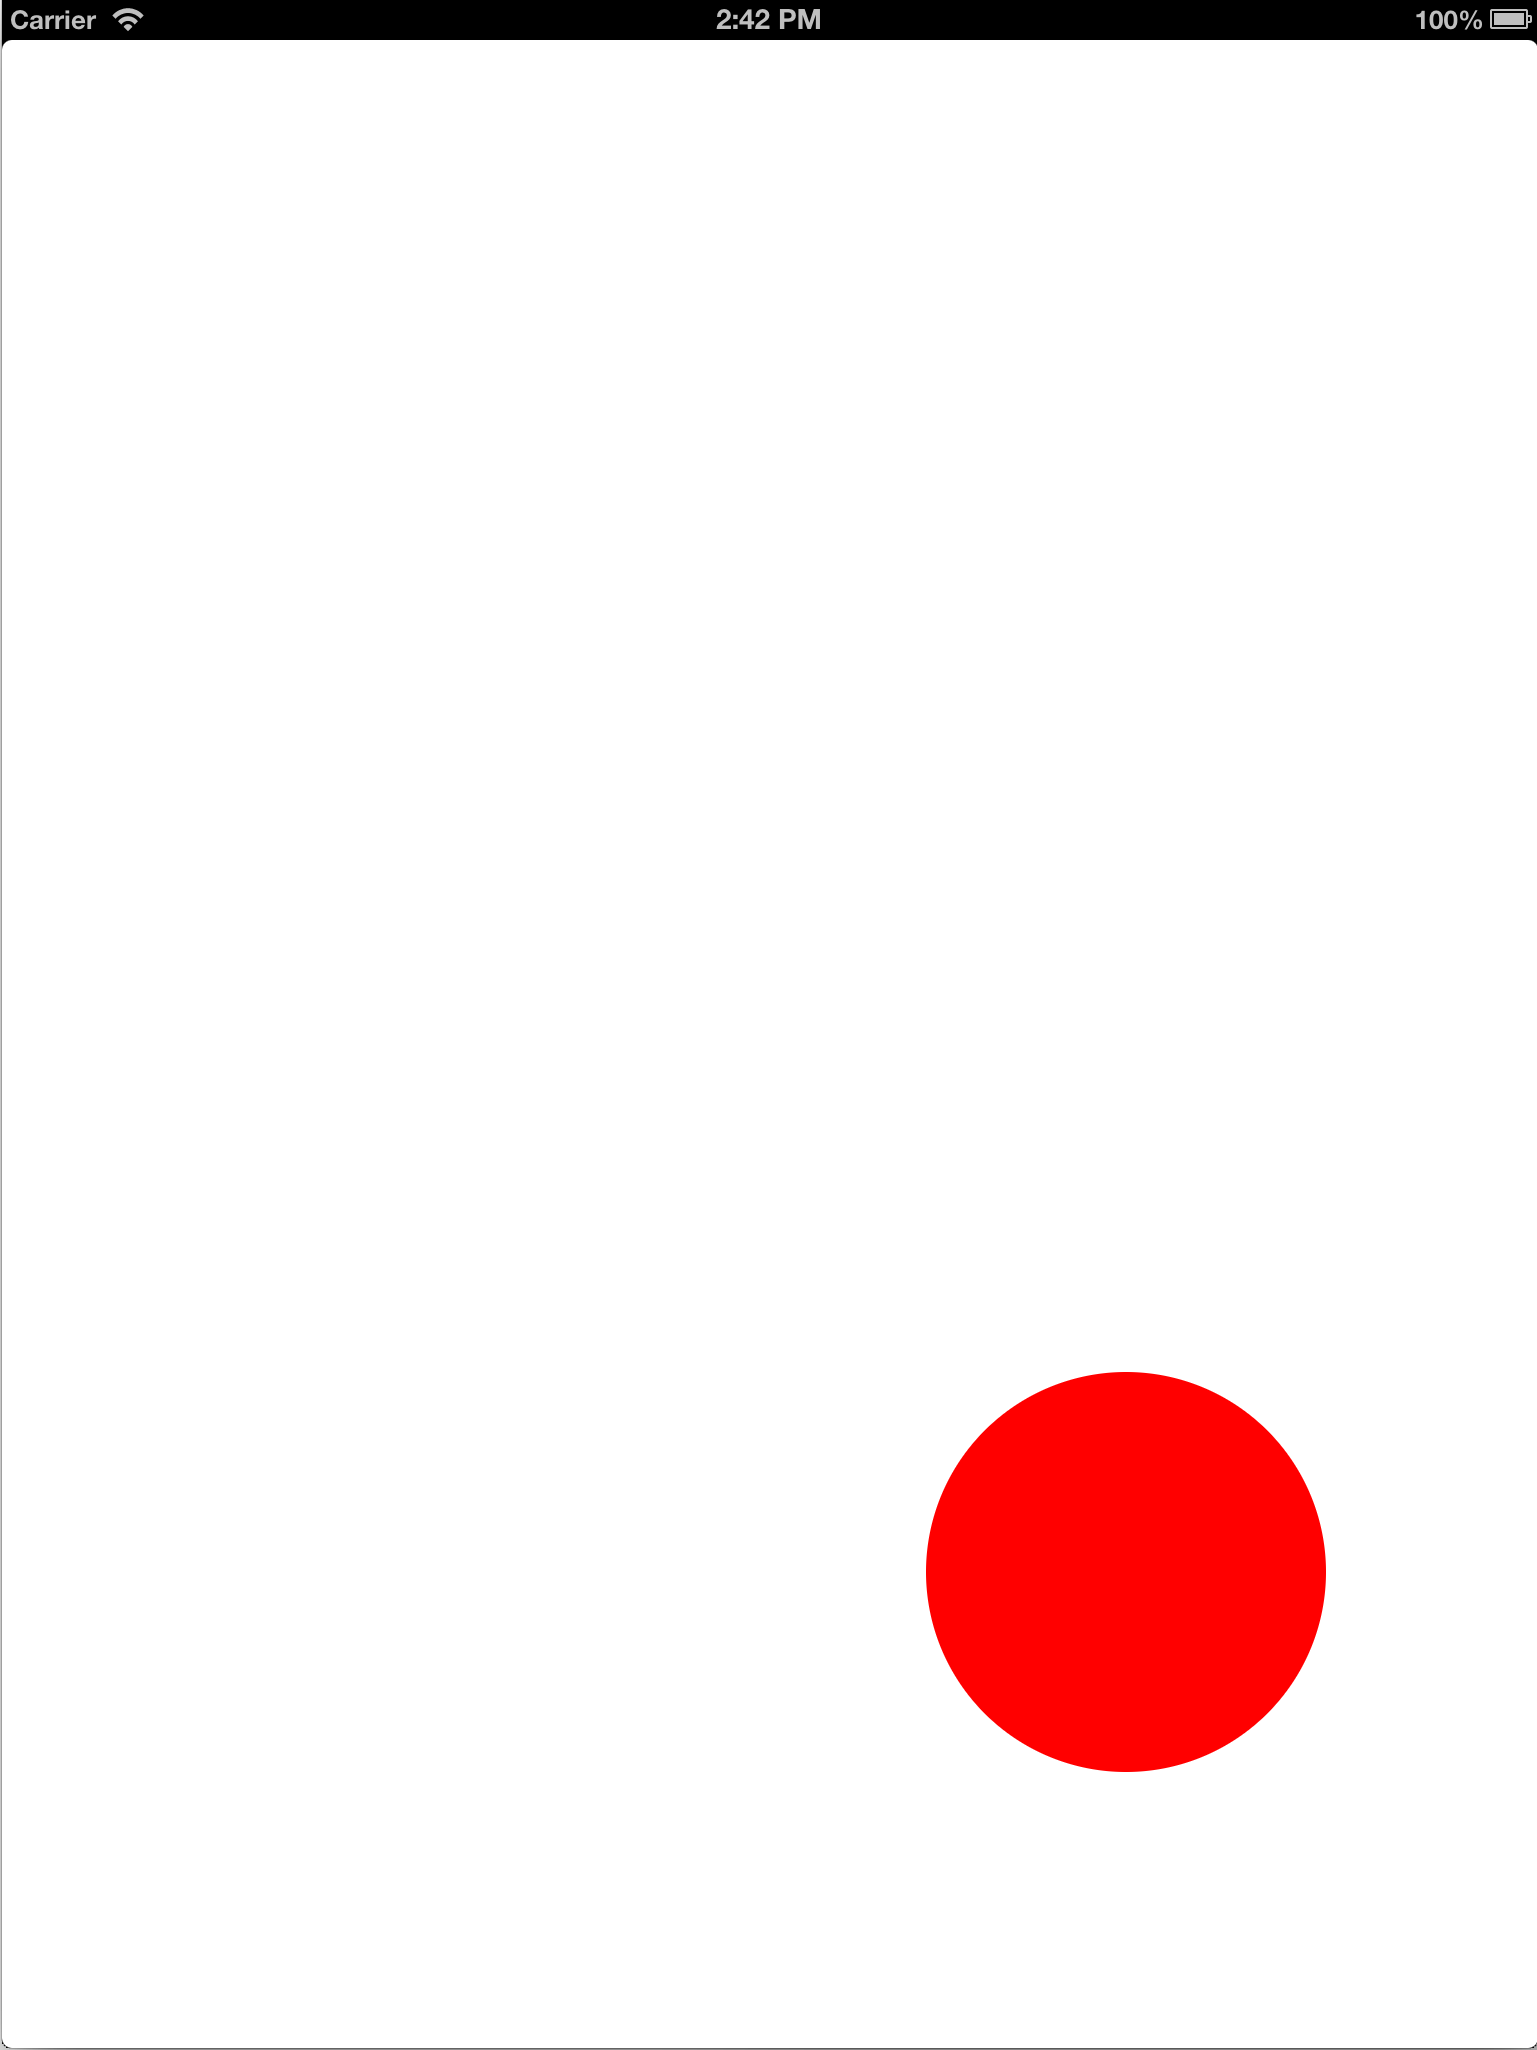
\includegraphics[width=0.45\textwidth]{test1}}}
\caption{\testfirst: in-game screenshot}
\end{figure}

\subsection{Balloon inflater}
\label{sec:test2}
The second test consisted of an application where the user was asked to inflate a balloon on the screen by tapping on it.
The balloon enlarged at every tap and shrank if not touched.
The resulting interaction is the user tapping repeatedly on the balloon in order to make it bigger, with the final result of making it explode as its dimension went beyond the screen bounds.

\begin{figure}[h!t]
\label{fig:experiment}
\centering
	{\setlength{\fboxsep}{0pt}
	 \fbox{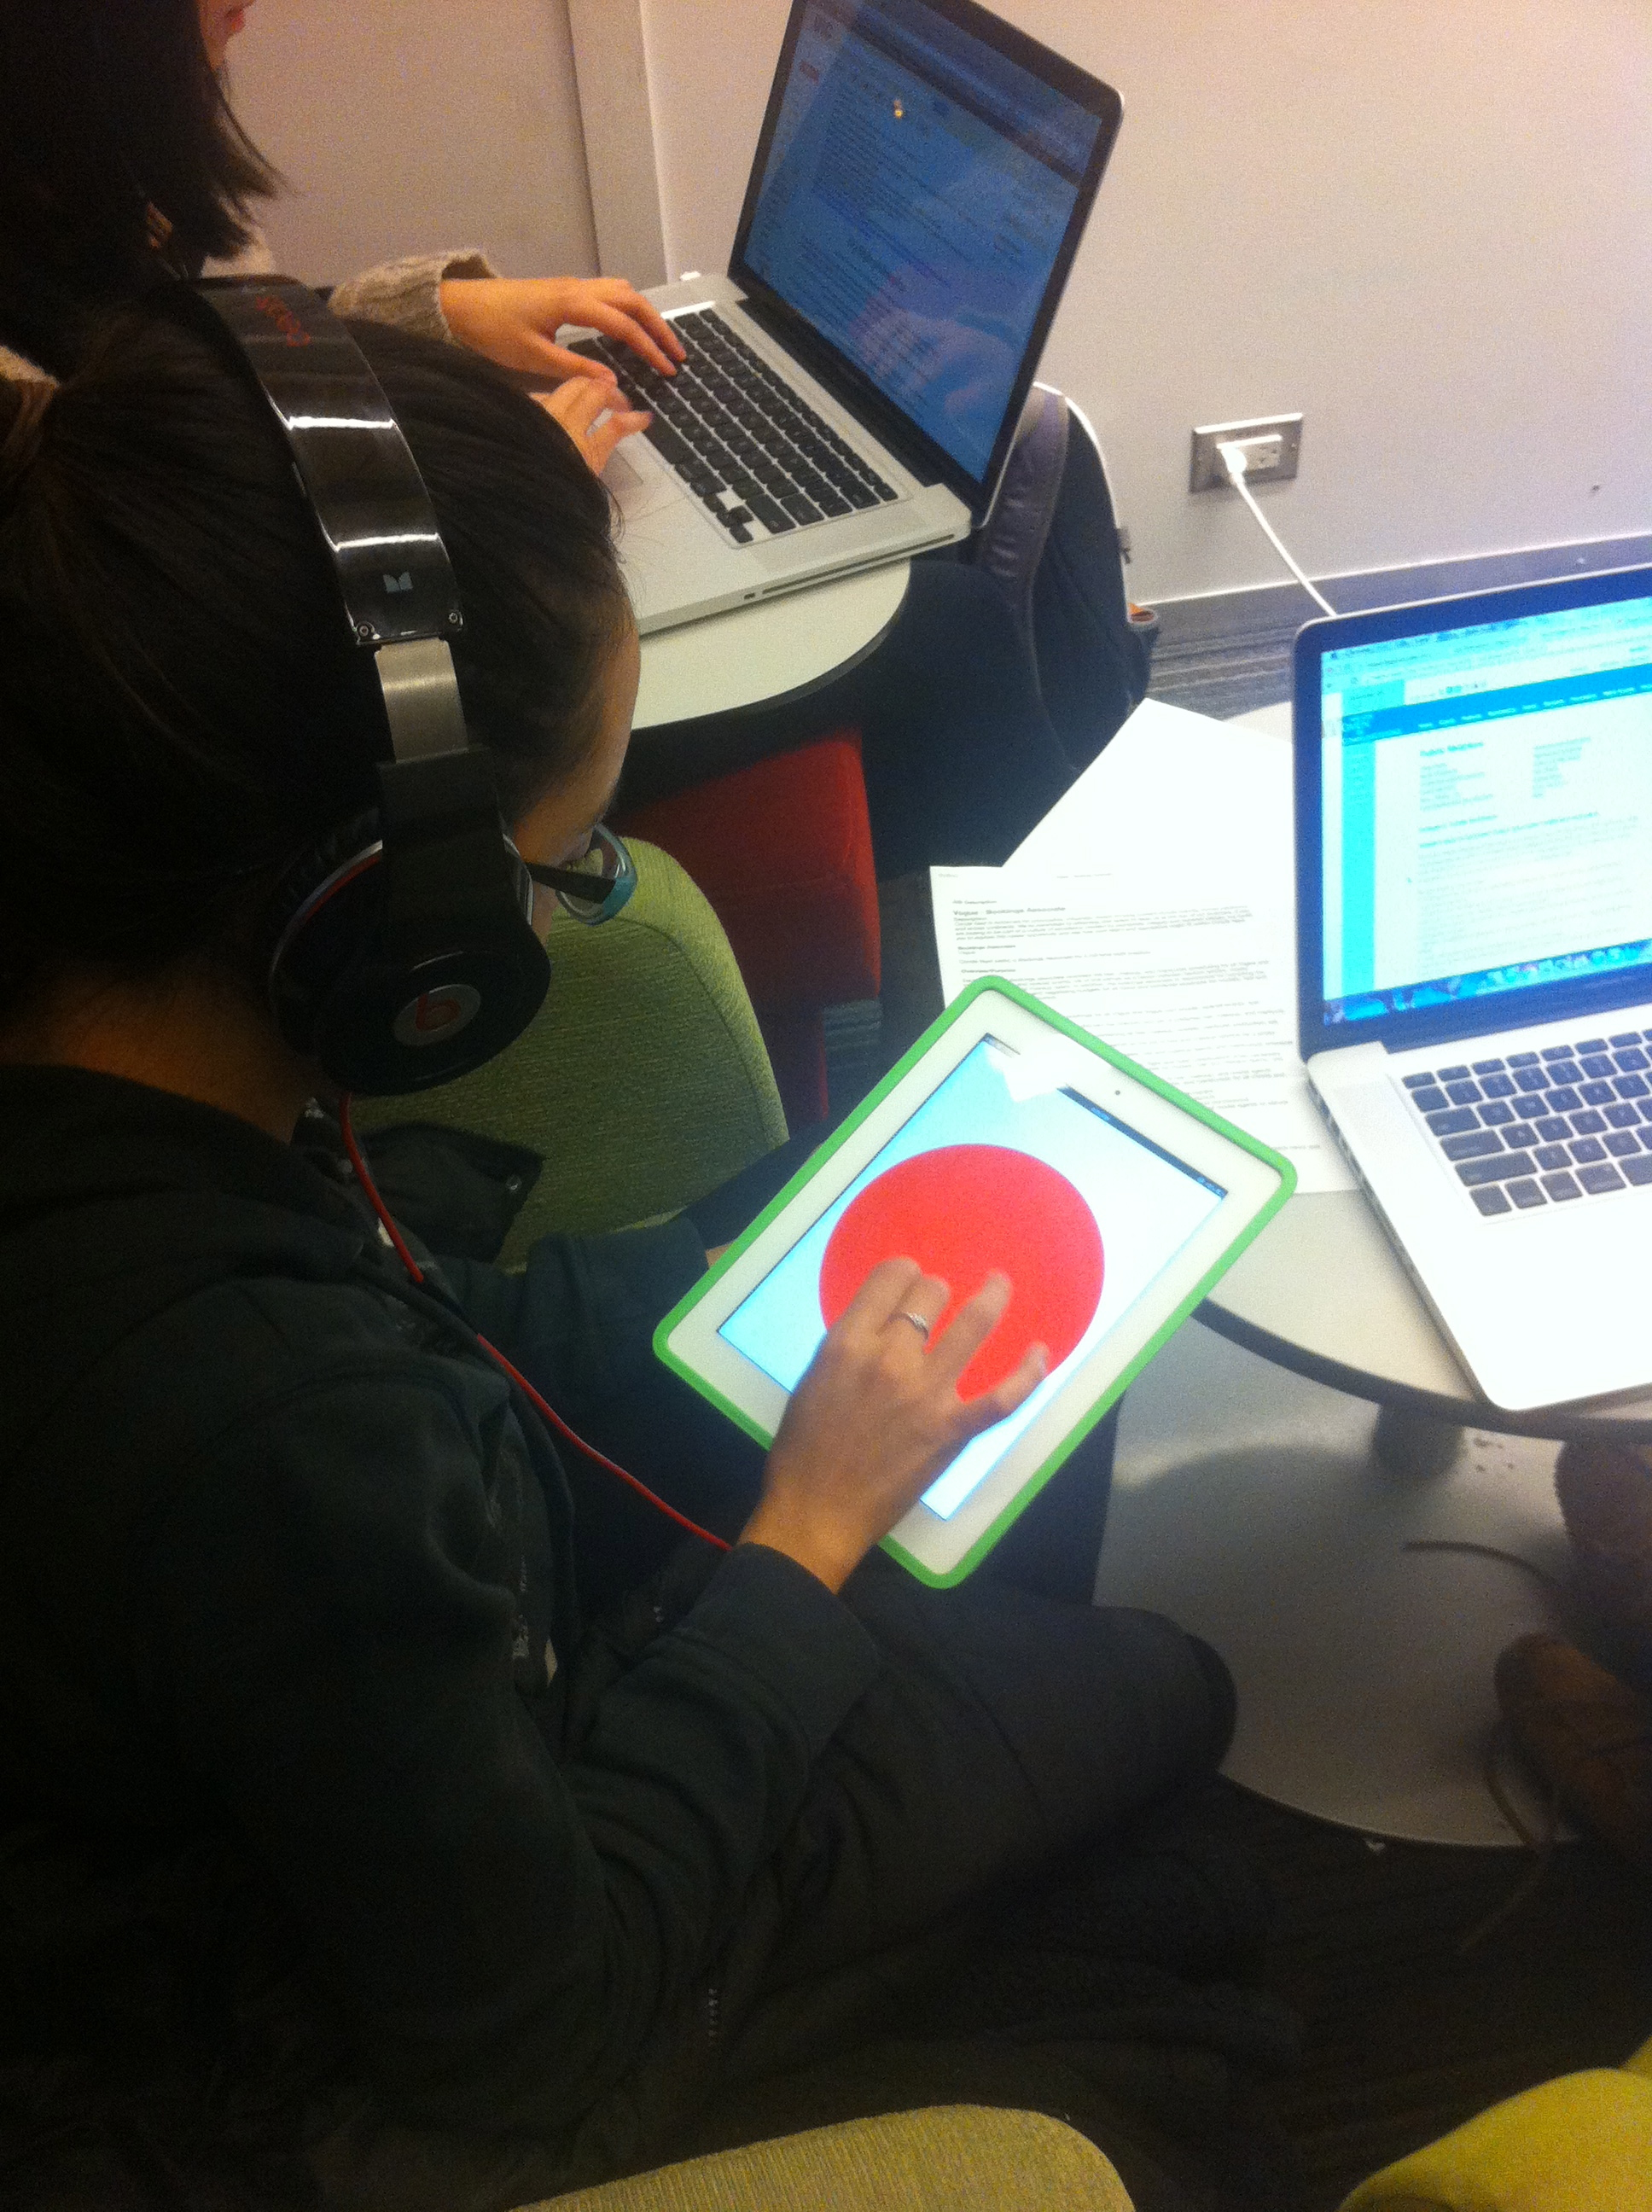
\includegraphics[width=0.45\textwidth]{experiment}}}
\caption{A tester in action}
\end{figure}

With respect to the previous test the interaction required much less cognitive activity, in the sense that the user concentration on the screen was not required in order to achieve the final result of exploding the balloon.

We will discusses later in Section~\ref{sec:conclusions} how this difference impacted on the test results.

\subsection{Data Collection}
Before moving on to the results we now present briefly how the data collection happened.

The iPad application was configured to send the data about the interaction of the user with the touchscreen to a web server we created specifically for this experiment. All the architecture has been implemented in JavaScript, taking advantage of the features of the framework Node.js.

In order to ensure that the collection was proceeding flawlessly, i.e. the data were being correctly sent to the web server, we decided to send and display them in real-time on a custom web page; the raw data were contextually stored on a MongoDB database.

The collection of raw data allowed us to avoid information loss and enabled us to perform further analysis on them.
% !TEX root = main.tex
\section{Performance evaluation}
In this section we now present the different performance measures adopted to evaluate the goodness of our goals.

\subsection{Experiment 1 - \testfirst}
In this test we want to measure the \emph{regularity} of the sequence of taps performed by the user. Moreover it is interesting to measure also the frequency synchronization w.r.t. the given beat and the \hl{``normalized'' synchronization}. \todo[color=yellow,inline]{Find a better name for this}
Let us now see how we defined such measures.
\subsubsection{Regularity}
For regularity we mean that the user should tap on the balloon at regular intervals. So a good regularity measure should be better when the time intervals are very similar to each other and bad when they are not. Therefore we decided to measure regularity as the \emph{mean squared error} (MSE) of the intervals between each user's tap.
The lower the error the better the regularity.
Thus the mathematical formulation will be
\begin{align}
	\frac{1}{n}\displaystyle\sum\limits_{i=0}^n(\bar{X}-X_i)^2
\end{align}
where $X_i$ is the ith time interval and $\bar{X}$ is the mean of the time intervals.

It is worth to notice that the regularity could be uncorrelated to the synchronization, in the sense that a user could produce a very regular sequence without being synchronized with the provided soundtrack.
\todo[inline,color=yellow]{Say something w.r.t to the data once we have them}

\subsubsection{Synchronization}
As stated above the regularity might be uncorrelated to the synchronization, so we also want to have a performance measure of the user synchronization with the provided soundtrack.
In order to achieve this for each beat interval we measure the delay between the user's tap and the last closest beat.
If no user's tap or more than one taps occur in the interval, we take as delay the whole distance between two consecutive beat.
\missingfigure{An image to explain the sync measure}
We then take the sum of every delay as the final measure.
The lower the sum the better the overall synchronization.

\subsubsection*{Normalized Synchronization}
As we already said, the user could be regular without being synchronized with the background music. However it may happen that the user is synchronized to a tempo which is $n$ times faster or slower than the given one.
In order to discover such a synchronization we decided to measure the ratio between the average time interval between user's taps and the regular interval of the soundtrack. The mathematical formalization for this is the following:
\begin{align}
	NormSync = \frac{\bar{X}}{T}
\end{align}
where $\bar{X}$ is the average time interval between user's taps and T is the interval between the soundtrack's beats.
If the number is close to an integer number and the user's sequence is regular then the user is likely synchronized to a multiple (or divisor) of the given tempo.
\missingfigure{A graph of the function}

\subsection{Experiment 2 - \testsecond}
% !TEX root = main.tex
\section{Results and findings}
We will now present the results of our experiments, going through each one of the already presented measures.

\subsection{Regularity}
As we stated before, the regularity tells us whether the users tend to be regular while tapping the red balloon during the activity. Let us first consider the first one, \testfirst. In Figure~\ref{fig:reg1} we can see the plot of the means squared error (from now on referred as MSE) for the activity. As we can see some sessions are very irregular in the beginning but all of them tend to a very low MSE, meaning that all the users are becoming very regular after a few seconds of activity. Besides of the observation of the graph this result is also confirmed by a very low average MSE of 0.15.

\todo[inline]{Unit measures on graphs. Also remove or mark the average line.}

\begin{figure}[h!t]
\centering
	{\setlength{\fboxsep}{1.5pt}
	 \fbox{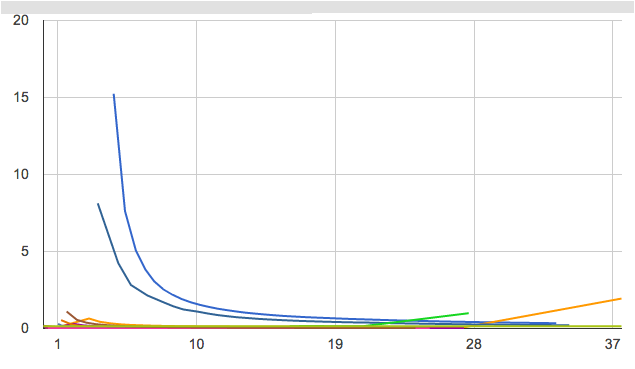
\includegraphics[width=0.45\textwidth]{reg1}}}
\caption{Regularity of \testfirst experiment}
\label{fig:reg1}
\end{figure}

On the other hand the MSE for the \testsecond experiment is very irregular, as shown in Figure~\ref{fig:reg2}, and does not tend to zero as the first one. We can observe that approximately for 5 seconds most of the users tend to tap regularly on the balloon, becoming then very irregular later on. This is probably due to the fact that during the first seconds of the activity they are trying to understand the balloon's behavior and when they get it they trying to inflate it as fast as they can, constantly increasing their tapping speed. This leads to very irregular tap intervals and a higher average MSE of 1.78.

\begin{figure}[h!t]
\centering
	{\setlength{\fboxsep}{1.5pt}
	 \fbox{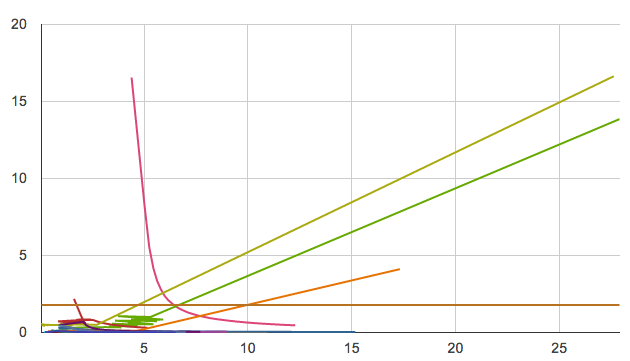
\includegraphics[width=0.45\textwidth]{reg2}}}
\caption{Regularity of \testsecond experiment}
\label{fig:reg2}
\end{figure}
% !TEX root = main.tex
\section{Conclusions}
\label{sec:conclusions}
We will now summarize the meaning of the results, that we already partially discussed during their presentation.

The consistent regularity, the good synchronization score and the synchronizatio ratio close to 1 indicate that the first test, \testfirst, enforces a good synchronization with the background tempo.

On the other hand an irregular tapping behavior, along with a poor synchronization score and a synchronization ratio far both of 0.68 (and therefore both far from the period, 1, and the half period, 0.5) indicate that in the second test, \testsecond, the background music is not affecting the behavior of the users in an appreciable way.

Thus, the synchronization is highly influenced by the kind of task and/or the background tempo. So far we identified three major components representing the main differences between the two experiments:

\begin{description}
	\item[Cognitive workload] While the \testfirst experiment required the user to stay focused on the activity in order to follow the balloon on the screen, the \testsecond experiment did not require any focus: one could have successfully completed the activity without even looking at the screen.

	Therefore theres is a well denoted difference between the two experiments in terms of cognitive workload required to perform the proposed activities.
straight-tunnel steering
	\item[Goal-driven] The \testfirst experiment was a potentially never-ending activity with a very regular and plain evolution (a balloon moving randomly around the screen without variating in shape or color). Therefore the user did not perceive any goal to reach neither implicit nor explicit. The \testsecond experiment, on the other hand, had an implicit goal-driven fashion. In fact, even if the users were not aware of the final explosion of the balloon, its inflation behavior suggested an evolution of the activity towards a critical point.

	This is another significant difference between the two activities

	\item[Tempo] In order to choose the BPM for each of the experiments we applied arbitrary variations to the natural BPM recorded in the bases case, as already discussed in Section~\ref{sec:basecases}. Specifically we decided to speed up the tempo for the \testfirst experiment and to slow it down for the \testsecond experiment.
	Such arbitrary decision introduced a difference between the two tests and therefore has to be accounted as a possible variable affecting the final results. 
\end{description}

Given our study it is not possible to discriminate and understand the importance of such variables over the final results that we presented above.

We will then discuss in Section~\ref{sec:future} which studies could be conducted in order to separate and weight the importance of each single variable, but all we can say so far is that the synchronization is probably affected by a convolution of those three variables.
% !TEX root = main.tex

\section{Future development}\label{sec:future}
As we discussed in the \nameref{sec:conclusions} section we identified a convolution of three variables that may have affected the final results of our study.
We will now discuss which studies could be conducted in order to separate and weight the importance of each single variable.

In order to understand the effect of the tempo's BPM would interesting to investigate whether a synchronization behavior can be reproduced with different BPMs and, if so, at which extent.
For instance we noticed that users synchronize at a 130 BPM tempo while performing the \testfirst activity, but we don't know whether they would to the same with a faster or slower tempo.
It is likely that there may exist one or multiple windows of BPMs for which a human subject tend to synchronize with the background music tempo, but it clearly needs to be extensively tested with actual data.
Setting the bounds of the effect we highlighted in our study could also help in applying it to real life situation, in which, as stated in the \nameref{sec:framing} section, may be useful to enforce a slower or faster behavior, e.g. in as video-games and work environments.

In order to understand instead the effect of the cognitive workload required an interesing experiment to conduct would be to variate it, keeping the other variables constant. For instance it could possible to set up an activity in which the cognitive workload required  is initially very low (like a tapping activity with a very big balloon, difficult to miss) and gradually increase it (for instance shrinking the size of the balloon).

A similar approach could be useful for investingating the effects of the presence of a implicit or explicit goal. One could set up an activity in which there's no goal at the beginning, \testfirst is a good example, and then gradually increase the goal requirements, for instance assigning an explicit score according to the number of performed taps or their precision.
Such an experiment could help in discovering whether the user tends to ignore the background music as soon as the goal requirements become more strict and evident.

% \balance

\nocite{*}
\bibliographystyle{acm-sigchi}
\bibliography{bibliography}

\end{document}